\textbf{Question 26.} \\
\hrule 

A certain system can experience three different types of defects. Let A, B and C denote the event that the system has a defect of each respective type. Suppose that 
\begin{align*}
    P(A) = .12 && P(B) = .07 && P(C) = .05 \\
    P(A \cup B) = .13 && P(A \cup C) = .14  && P(B \cup C) = .10 \\
    P(A \cap B \cap C) = .01
\end{align*}

Before we even tackle the given problems we us calculate our intersections so we can create a Venn diagram. That will make this very smooth for us. We'll be using the general addition rule as usual.
\begin{align*}
    P(A \cap B) &= P(A) + P(B) - P(A \cup B) \\
    P(A \cap B) &= .12 + .07 - .13 \\
    P(A \cap B) &= .06
\end{align*}
A similar strategy is used for the other two intersections which resulted in $P(A \cap C) = .03$ and $P(B \cap C) = .02$. From here we can create our diagram and we take note of our given triple intersection value when putting in our other intersections.

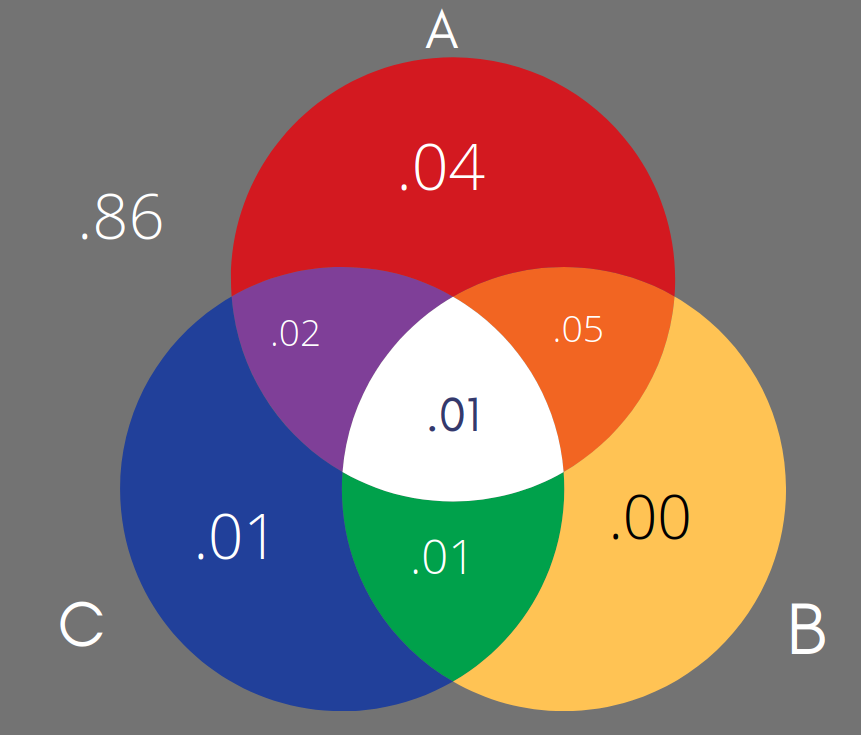
\includegraphics[scale=0.25]{images/whw3/2.2.26_venn.png}

Now we can easily answer any questions provided. 

\textbf{a. What is the probability that the system does not have a type A defect?} \newline 
We simply need to subtract out .12 from 1 to remove all type A defects from our probability. This gives us $\boxed{.88}$

\textbf{b. What is the probability that the system has both type A and type B defects?} \newline 
We can use our calculation for $P(A \cap B)$ here which was $\boxed{.06}$. 

\textbf{c. What is the probability that the system has both type A and type B defects but not a type C defect?} \newline
This can be defined as $P((A \cap B) \cap C')$. This is simply .06 from part (b) minus .01 from our triple intersection. The answer is $\boxed{.05}$. 

\textbf{d. What is the probability that the system has at most two of these defects?} \newline 
This one is deceptively simple. Since the highest amount of defects we can have is 2, we just subtract out the probability that we get all 3 defects. Our answer here is $\boxed{0.99}$.
